\newSec[Arch]{Software-Architektur}{1}

In diesem Kapitel soll die Architektur des Projekts umrissen werden. 


\newSec[ArchConcept]{Architektur Konzept}{2}
Der Aufbau der Architektur entspricht den Konzept der \clean. Diesem Prinzip folgend zeigen sämtliche Abhängigkeiten des Codes auf \textit{weiter innen liegende} Schichten.
Die Farbgebung in \refImg{fig:Arch} orientiert sich an den Inhalten der Vorlesung \texttt{Advanced Software-Engineering} der \DHBW.




\begin{figure}[ht!]
\vspace{0.25cm}
\begin{center}
\fbox{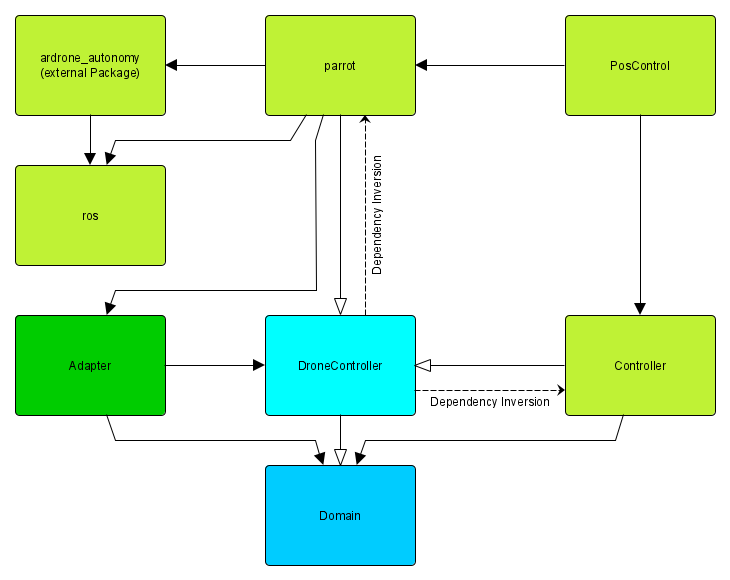
\includegraphics[width=15cm]{Pictures/Architecture Blocks.png}}
\caption{Architektur des Positionsregelungssystems}
\label{fig:Arch}
\end{center}

\vspace{0.25cm}
\refImgShort{fig:Arch} zeigt das Konzept der Architektur. Die Bedeutungen der Pfeile orientieren sich an UML-Klassendiagrammen. Die Farbgebung unterscheidet die verschiedenen Schichten der \clean: \textit{Domain-Layer} (blau), \textit{Application-Layer} (hellblau), \textit{Adapter-Layer} (grün), \textit{PlugIn-Layer} (hellgrün).
\end{figure}





\newSec[ArchDomain]{\textit{Domain} \Pack}{2}





\newSec[ArchDrone]{\textit{DroneController} \Pack}{2}
Das Entwurfsmuster des \textit{Application-Layer} entspricht einer \textit{Bridge}. Ziel ist es, sowohl die eingesetzte Drohne, als auch die Implementierung des Reglers mit überschaubarem Aufwand austauschen zu können.

Ferner wird in diesem \Pack


\newSec[ArchAdapter]{\textit{Adapter} \Pack}{2}






\newSec[ArchController]{\textit{Controller} \Pack}{2}






\newSec[ArchParrot]{\textit{parrot} \Pack}{2}




\newSec[ArchPosControl]{\textit{PosControl} \Pack}{2}